\documentclass{article}
\usepackage{graphicx}
\usepackage{hyperref}
\usepackage{amsmath}
\usepackage{enumitem}

\title{LLM Anonymization Techniques Recommender for Datasets (LLMANO-2)}
\author{Amin Akziz, Leander Ziehm, Azbabanu Engineer, Santiago Lema}
\date{July 2025}

\usepackage[a4paper, margin=1in]{geometry}

\usepackage{setspace}
\onehalfspacing

\begin{document}

\maketitle

\begin{center}
\begin{minipage}{0.85\textwidth}
\section*{Abstract}
The need for anonymizing datasets has grown significantly with the proliferation of machine learning and large language models (LLMs). However, many users lack a clear understanding of how to properly anonymize their data without significantly compromising its utility. In response to this challenge, we present LLMANO-2, a recommender system that leverages LLMs to guide users in anonymizing CSV datasets while preserving predictive performance. Our system provides tailored recommendations based on the specific characteristics of each dataset, aiming to strike a balance between privacy and usability. The motivation for this work stems from recent data privacy incidents that highlight the risks of improper anonymization and the growing demand for practical, intelligent tools to support privacy-aware data publishing.
\end{minipage}
\end{center}

\section{Introduction}

In today’s era of big data and artificial intelligence, vast amounts of personal and sensitive information are being collected and analyzed. This increase in data collection has made dataset anonymization a critical concern, as organizations must protect individual privacy while still deriving value from the data.

Notably, data anonymization is not just a best practice but often a legal requirement, privacy regulations like the EU’s General Data Protection Regulation (GDPR) and the California Consumer Privacy Act (CCPA) mandate that personal data be anonymized or otherwise protected if it’s to be used beyond its original purpose. Failure to properly anonymize data can lead to severe regulatory penalties as well as loss of user trust.

Recently, advances in Artificial Intelligence have introduced new possibilities for smarter anonymization approaches. In particular, Large Language Models (LLMs) offer a promising approach to tackle the privacy-utility trade-off. In alignment with these developments, our work proposes LLMANO-2, an LLM-powered anonymization technique based recommender for datasets. LLMANO-2 is designed to assist users in anonymizing tabular datasets by recommending appropriate techniques for each column of data. For a given dataset, the system leverages an LLM to analyze the column contents and identify which fields are likely sensitive and suggest how to transform or mask them. The recommendations aim to maximize privacy protection while minimizing the impact on the dataset’s utility for analysis or machine learning tasks. In the following sections we describe the architecture and methodology behind LLMANO-2, including how it processes datasets, generates anonymization recommendations, and evaluates the effectiveness of those recommendations.


\section{Background and Theory}

A dataset (for example, a CSV file or database table) typically consists of many records (rows) with multiple attributes (columns) describing each record. These attributes can include direct identifiers (such as names, email addresses, or national ID numbers) as well as indirect identifiers (such as dates of birth, gender, or ZIP codes) that might not identify someone on their own, but could do so when combined with other information.

Data anonymization refers to the process of modifying a dataset to remove or obscure personal identifiers so that individuals cannot be readily identified. It involves erasing or encrypting identifiers that connect an individual to stored data while retaining the data’s overall usefulness. The challenge is to ensure privacy without significantly degrading the utility of the data.

In practice, anonymization techniques may include removing or masking direct personal identifiers, generalizing values (for example, replacing an exact age with an age range), or pseudonymizing data by replacing real identifiers with artificial codes. These transformations allow organizations to use data for insights without exposing specific individuals.

\begin{figure}[h]
    \centering
    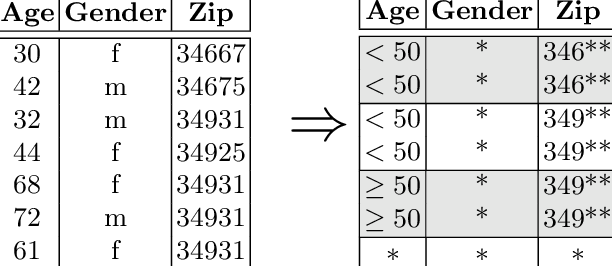
\includegraphics[width=0.65\linewidth]{images/figure1.png}
    \caption{Example of an anonymization technique applied to a simple dataset}
    \label{fig:anonymization-example}
\end{figure}

This is especially important when sharing datasets with third parties or releasing them publicly for research, as it enables data sharing and collaboration without compromising confidentiality.

Despite its importance, effective anonymization can be challenging. Research has shown that improperly anonymized datasets can still compromise privacy. Certain attributes are extremely sensitive, and even "anonymized" data can be re-identified. A famous statistic by Latanya Sweeney demonstrated that 87\% of the U.S. population could be uniquely identified using only three pieces of information, birth date, gender, and ZIP code, highlighting how a few quasi-identifiers can pinpoint individuals.

Another example where personal data was compromised is in the Netflix Prize dataset released in 2006, which contained movie ratings with personal identities removed, researchers were able to re-identify specific users by correlating the anonymized ratings with public information on IMDb (Internet Movie Database). This meant that personal viewing preferences (and even sensitive attributes inferred from them) of certain Netflix users became public, despite Netflix’s attempt to anonymize the data.

These cases show that simply removing obvious identifiers is often not sufficient. If enough data remains, determined adversaries can link supposedly anonymous records back to real individuals. Beyond the harm to individuals (such as exposing health information, financial status, or location history), such incidents expose organizations to legal liabilities and reputational damage. As data mining and cross-referencing techniques grow more sophisticated, re-identification attacks are becoming easier and more common. This puts pressure on data publishers to adopt stronger anonymization measures than were needed in the past.

At the same time, anonymization must be done carefully to preserve the usefulness of data. Over-aggressive anonymization, such as deleting or randomizing too many fields, can render a dataset nearly useless for analysis or model training, defeating the purpose of sharing the data. The more we strip away or distort to protect privacy, the less accurate or insightful the dataset becomes. A core challenge is finding the sweet spot where sensitive details are well-protected, yet the dataset still supports meaningful insights or predictions.

Achieving this balance often requires expertise and context, deciding which attributes to generalize or mask, and to what extent, without degrading the data’s integrity. Unfortunately, many users and organizations lack a clear understanding of how to achieve this. Choosing the right anonymization techniques depends on the data content, possible auxiliary data an attacker may use, and the intended use of the anonymized dataset. As a result, there is a growing need for tools and guidance to help data owners navigate this complexity.

------------------------------------------------------------------------------------------------------------------------------------

\begin{itemize}
\item \textbf{Direct identifiers} (e.g., names, emails)
\item \textbf{Quasi-identifiers} (e.g., weight, height, age)
\item \textbf{Anonymity metrics} such as $k$-Anonymity, $l$-Diversity, and $t$-Closeness
\item \textbf{Anonymization Methods}
\end{itemize}

We also discuss user-driven anonymization processes and the limitations of manual or rule-based methods in ensuring privacy. In the remainder of this section, we outline the mathematical foundations underlying key privacy-preserving techniques in data publishing, including $k$-anonymity, $l$-diversity, and generalization strategies.

\subsection{Identifiers and Quasi-Identifiers}

In the context of privacy-preserving data analysis, it is essential to distinguish between different types of attributes:

\begin{itemize}
\item \textbf{Direct Identifiers} are attributes that can uniquely identify an individual without external information. Common examples include names, social security numbers, or email addresses.

\item \textbf{Indirect Identifiers}, also called \textit{quasi-identifiers}, are attributes that do not uniquely identify an individual on their own but can do so when combined with other quasi-identifiers. Examples include age, ZIP code, and gender.
\end{itemize}

Effective anonymization techniques aim to remove or transform these identifiers such that the risk of re-identification is minimized.

\subsection{$k$-Anonymity}

The concept of $k$-anonymity, introduced by Sweeney, is one of the foundational principles for privacy protection. A dataset is said to satisfy \textbf{$k$-anonymity} if each record is indistinguishable from at least $k-1$ other records with respect to the quasi-identifiers.

Formally, given a dataset $D$ with quasi-identifier attributes $Q_1, Q_2, ..., Q_m$, let $\pi$ be a projection onto the quasi-identifier space:

$$
\pi(D) = \{ (q_1, q_2, ..., q_m) \mid (q_1, ..., q_m) \in D \}
$$

Let $E$ be an equivalence class of records in $D$ that share the same quasi-identifier values:

$$
E = \{ r \in D \mid \forall i, \; r[Q_i] = v_i \}
$$

Then $D$ satisfies $k$-anonymity if:

$$
\forall E \subseteq D, \quad |E| \geq k
$$

This ensures that an adversary can not link any given record to fewer than $k$ individuals. However, $k$-anonymity alone does not prevent \textit{attribute disclosure}—when sensitive values within a group are too homogeneous.

\subsection{$l$-Diversity }

$l$-Diversity extends $k$-anonymity to protect against attribute disclosure by ensuring that each equivalence class has at least $l$ ``well-represented'' sensitive attribute values.

\paragraph{ Definition.}
An equivalence class $E$ is said to have \textit{distinct $l$-diversity} if it contains at least $l$ distinct values for the sensitive attribute $S$:

\[
|\{ s_i \mid s_i \in E \}| \geq l
\]

where $s_i$ denotes the sensitive value of record $i$ in equivalence class $E$.

\paragraph{Variants.}
\begin{itemize}
    \item \textbf{Distinct $l$-diversity:}
    \[
    |\{ s_i \}| \geq l
    \]
    Requires at least $l$ distinct sensitive values, regardless of their distribution or meaning.

    \item \textbf{Entropy $l$-diversity:}
    Defines diversity using entropy of the sensitive value distribution within $E$:
    \[
    H(E) = - \sum_{s \in S} p_s \log p_s \geq \log l
    \]
    where $p_s$ is the fraction of records in $E$ with sensitive value $s$. This ensures a balanced distribution.

    \item \textbf{Recursive (c, $l$)-diversity:}
    Limits the dominance of the most frequent sensitive value. Formally, for the sorted frequencies $f_1, f_2, ..., f_m$:
    \[
    f_1 < c \cdot (f_l + f_{l+1} + ... + f_m)
    \]
    where $c$ is a parameter controlling strictness. This prevents a single sensitive value from overwhelming others even if there are $l$ distinct values.
\end{itemize}

\paragraph{Why Needed.}
While $k$-anonymity prevents identity disclosure, it does not prevent attribute disclosure if all records in an equivalence class share the same sensitive value. $l$-Diversity mitigates this by ensuring diversity in sensitive attributes.

\paragraph{Limitations.}
\begin{enumerate}
    \item \textbf{Skewness Attack.} If the overall distribution is skewed (e.g. 99\% flu, 1\% cancer), $l$-diversity fails to prevent inference because the presence of rare values remains revealing.

    \item \textbf{Similarity Attack.} Even if an equivalence class has $l$ distinct sensitive values, if they are semantically similar (e.g. different types of cancer), meaningful privacy is not protected.
\end{enumerate}


\subsection{$t$-Closeness }

$t$-Closeness improves upon $l$-diversity by protecting against attribute disclosure through distributional similarity constraints.
\paragraph{ Definition.}
An equivalence class $E$ is said to have \textit{$t$-closeness} if the distance between the distribution of the sensitive attribute within $E$ ($P_E$) and the global distribution ($P_T$) is no more than a threshold $t$:

\[
D(P_E, P_T) \le t
\]

where:
\begin{itemize}
    \item $P_E$ is the probability distribution of sensitive attribute values in equivalence class $E$
    \item $P_T$ is the global distribution of the sensitive attribute in the entire dataset
    \item $D(\cdot)$ is a chosen distance measure, typically Earth Mover's Distance (EMD) or Kullback-Leibler Divergence.
\end{itemize}

\paragraph{Motivation.}
$l$-Diversity fails if equivalence class distributions are skewed compared to the overall data, enabling attribute inference attacks. $t$-Closeness mitigates this by bounding the distributional distance.

\paragraph{Common Distance Measures.}
\begin{itemize}
    \item \textbf{Earth Mover's Distance (EMD):} Measures the minimum amount of ``work'' required to transform one distribution into another, considering attribute semantics. It is formally defined as:
    \[
    EMD(P_E, P_T) = \inf_{\gamma \in \Gamma(P_E, P_T)} \int |x-y| d\gamma(x,y)
    \]
    where $\Gamma(P_E, P_T)$ is the set of all joint distributions with marginals $P_E$ and $P_T$.

    \item \textbf{Kullback-Leibler (KL) Divergence:}
    \[
    D_{KL}(P_E || P_T) = \sum_{i} p_E(i) \log \frac{p_E(i)}{p_T(i)}
    \]
    Note: KL-divergence is asymmetric and unbounded, limiting its practical use in $t$-closeness.

\end{itemize}

\paragraph{Example.}
If the global distribution is:
\[
P_T = \{ \text{Disease A}: 95\%, \text{Disease B}: 5\% \}
\]
but an equivalence class $E$ has:
\[
P_E = \{ \text{Disease B}: 100\% \}
\]
then even with $l$-diversity, an attacker learns an individual's disease with certainty. $t$-Closeness prevents this by ensuring $P_E$ remains close to $P_T$ within threshold $t$.

\paragraph{Advantages.}
\begin{itemize}
    \item Addresses both identity and attribute disclosure by enforcing global distribution similarity.
    \item Reduces risk of skewness and similarity attacks inherent to $l$-diversity.
\end{itemize}

\paragraph{Limitations.}
\begin{enumerate}
    \item \textbf{Utility Loss:} Strict $t$-closeness often requires heavy generalization or suppression, degrading data utility.
    \item \textbf{Threshold Selection:} Choosing an appropriate $t$ balancing privacy and utility is challenging.
    \item \textbf{Implementation Complexity:} Calculating EMD for categorical attributes requires defining semantic distances or hierarchies between categories.
    \item \textbf{Overprotection:} May restrict data utility disproportionately compared to marginal privacy gains in some contexts.
\end{enumerate}



\subsection{Anonymization Methods}
We summarize several key anonymization techniques, each suited to different data contexts and privacy requirements.

\textbf{Suppression} involves fully removing specific cells or rows from a dataset. It is most suitable for quick removal of extremely sensitive data, especially in open-data publication settings.

\textbf{Generalization} clusters records and replaces each cluster with a representative centroid or more general category. This method is particularly effective for numerical data and statistical summaries and supports privacy models such as $k$-Anonymity and $l$-Diversity. It is often used when preparing datasets for open-data release.

\textbf{Differential Privacy (Global, DP-SGD)} relies on query-based data release mechanisms where calibrated noise is added to the output. It is best suited for machine learning training (e.g., with DP-SGD) and interactive analytics, where a defined privacy budget (e.g., epsilon, delta) must be managed.

\textbf{Differential Privacy (Local)} applies privacy-preserving noise at the individual data record level before data collection. This method is ideal for decentralized or mobile data gathering scenarios, such as collaborative research with privacy guarantees at the point of data generation.

\textbf{Pseudonymization} replaces identifiers with consistent tokens, allowing data to remain linkable while obscuring personally identifiable information. It is often applied for regulatory compliance purposes.

\textbf{Tokenization} substitutes identifiers with cryptographic tokens and may leverage secure multiparty computation techniques. It enables privacy-preserving collaborative analysis and is well-suited for research collaboration contexts.

In addition to these methods, \textbf{homomorphic encryption} offers another avenue for privacy-preserving computation, allowing data to be processed while still encrypted. This enables secure computation without ever revealing the underlying sensitive values.

AGAIN CAN DELETE: Generalization

Achieving $k$-anonymity and $l$-diversity typically requires generalization and/or suppression of quasi-identifier attributes. Generalization replaces specific values with broader categories. For example:
\begin{itemize}
\item Age: 23 $\rightarrow$ [21--30]
\item ZIP Code: 12345 $\rightarrow$ 123**
\end{itemize}
more here todo leander.


The goal is to form equivalence classes with sufficient cardinality and sensitive attribute diversity, while minimizing information loss.





\section{Architecture}
\begin{itemize}
    \item Setup and hardware needed
    \item Overview diagram of system components
    \item LLM interface and decision flow
    \item Form interface for user inputs (direct/quasi identifier tagging)
    \item Backend anonymization and evaluation pipeline
\end{itemize}

\section{Related Work}
\subsection{Application of LLM-Assisted Deductive Coding for Fuzzy Matching}

In our system, we implemented a \texttt{fuzzy\_match} function inspired by the deductive coding approach presented by Arnold et al. (2023) in \textit{LLM-Assisted Content Analysis}. Their methodology uses large language models (LLMs) to select a single best-fitting label from multiple predefined options, grounded in context and code definitions. We adapted this technique for robust, scalable option selection tasks in our pipeline.

\subsubsection{How We Used the Technique}

\paragraph{Problem Context}
Our task required selecting the most appropriate code or label for a given candidate input, from a predefined set of options, based on its meaning within a specific context. This is conceptually identical to deductive coding, where text data is categorized using an established codebook.

\paragraph{Inspiration from the Paper}
The paper demonstrated that LLMs perform effectively when prompted with:
\begin{itemize}
    \item An input text
    \item A list of options (codes) with clear definitions and examples
    \item Instructions to select the best fitting option only from the list
\end{itemize}
This structured prompt ensures the LLM leverages its semantic understanding to perform closed-set classification, avoiding invalid or out-of-scope outputs.

\paragraph{Our Implementation}
In our \texttt{fuzzy\_match} tool:
\begin{itemize}
    \item We provide the model with:
    \begin{itemize}
        \item A \textbf{context} explaining the selection task
        \item The \textbf{options dictionary}, mapping each code to its definition
        \item The \textbf{candidate input} requiring classification
    \end{itemize}
    \item We construct a structured prompt instructing the model to select the correct code strictly from the provided options.
    \item The LLM generates a JSON response containing:
    \begin{itemize}
        \item The selected \textbf{code}
        \item An optional \textbf{rationale} explaining its choice
    \end{itemize}
\end{itemize}

This mirrors the paper's method, where the LLM’s reasoning is grounded in the definitions and examples given for each code, allowing it to perform classification based on semantic alignment rather than purely lexical similarity.

\subsubsection{Key Principle Applied}


\textbf{Closed-set selection with definitions.} The technique enforces that the output is always within the valid set of codes, ensuring interpretability, consistency, and compatibility with downstream processing pipelines. This is critical for tasks such as qualitative coding, label assignment, or controlled classification where outputs outside the predefined set are invalid.

\subsection{Inspiration from JarviX}

Our LLMANO‑2 system draws inspiration from \textit{JarviX} , a no-code platform for tabular data analytics using LLMs. JarviX elegantly combines structured workflows, prompt-engineering logic, and AutoML integration to guide users through complex analytic tasks. We adopted several of its key design elements:

\begin{itemize}
    \item \textbf{LLM-driven, context-aware prompt flow.} As in JarviX, our system assesses the dataset schema and user goals to generate guiding questions and suggest relevant next actions dynamically .

    \item \textbf{Missing-context queries.} When crucial information is not provided, LLMANO‑2 automatically asks follow-up questions—mirroring JarviX’s Question Matcher module that detects ambiguity and clarifies requirements before analysis execution.
    \item \textbf{Future prompt suggestions.} Inspired by JarviX’s Analysis Consultant, which recommends subsequent lines of inquiry and visualizations, LLMANO‑2 likewise offers users a menu of potential follow-up prompts to deepen insight.
    \item \textbf{Hierarchical system architecture.} We adopted a modular architecture similar to JarviX’s pipeline decomposition—starting from data ingestion, to LLM-driven interpretation, to visualization and optimization—enabling flexible extension and improved maintainability.
\end{itemize}

\paragraph{Workflow (adapted from JarviX).}
...............


\paragraph{Prompt logic.}
Let $\mathcal{D}$ be the dataset schema and $u$ the user's initial prompt. JarviX first derives:
\[
\mathrm{ctx}_0 = \textit{Parser}(\mathcal{D}, u),
\]
then checks completeness:
\[
\textit{if } \mathrm{ctx}_0 \not\vdash \textit{sufficient} \text{ then ask }\Delta q,
\]
and iterates until $\mathrm{ctx}_k$ is sufficient. The final query is submitted to the LLM for execution. This controlled, looped clarification inspired our back-and-forth logic.

\paragraph{Summary.}
By adapting JarviX’s workflow, prompt refinement, and suggestion strategies, LLMANO‑2 gains structured dialog management and context-sensitive prompting—key to robust no-code analytics. We extended this foundation with advanced context tracking and conversational capabilities to enhance usability and reliability.
\subsection{Definitions and Notation Used in LLMANO (Based on SCORR)}

In developing LLMANO, we adopted the definitions, notation conventions, and assumptions from the paper \emph{Scoring System for Quantifying the Privacy in Re-Identification of Tabular Datasets (SCORR)} . Specifically, we use its classification of Direct Identifiers (DIs), Quasi-Identifiers (QIs), and Sensitive Attributes (SAs), as well as its formal dataset notation and risk analysis assumptions.

\paragraph{Notation.}
Let $n$ be the number of records, $m$ the number of QI attributes, and $p$ the number of distinct persons:
\[
\begin{array}{rl}
\text{Attributes} &= \{a_1, a_2, \ldots, a_{m+2}\} \\
\text{Person ID} &= a_1 \\
\text{QI} &= \{a_2, \ldots, a_{m+1}\} \\
\text{SA} &= a_{m+2}
\end{array}
\]
where $v_{ij}$ is the value of attribute $a_j$ in record $i$, with:
\[
\begin{array}{rl}
v_{i1} &= u_k \quad \text{(Person ID)} \\
QI_i &= \{v_{i2}, \ldots, v_{i,m+1}\} \\
SA_i &= v_{i,m+2}.
\end{array}
\]

\paragraph{Assumptions.}
LLMANO adopts SCORR’s assumptions that:
\begin{enumerate}
    \item The intruder knows the QI values of the target data subject.
    \item The intruder aims to infer the SA value associated with the target.
\end{enumerate}

\paragraph{Summary.}
These definitions, notation structures, and assumptions from \emph{Scoring System for Quantifying the Privacy in Re-Identification of Tabular Datasets} provide the foundation for LLMANO’s identifier recognition logic, privacy metric calculations, and risk analysis modules.

\section{Evaluation}
Our system allows users to:
\begin{enumerate}
    \item Upload CSV datasets
    \item Select columns as direct or quasi-identifiers (form includes definitions and examples)
    \item Receive LLM-generated anonymization recommendations (e.g., $k=10$)
    \item Optionally adjust granularity and generalization steps
\end{enumerate}
LLMs are prompted to recommend anonymization strategies based on dataset structure and user inputs. Screenshots and/or GitHub links will be included.

We test our system on multiple datasets:
\begin{itemize}
    \item Comparison against human-created anonymization
    \item Benchmarking against other anonymization algorithms
    \item Metrics: preservation of predictive accuracy, anonymity scores
\end{itemize}
Each configuration is tested 10 times to compute average performance. Evaluation is automated and requires no user interaction.

\section{Limitations, Discussion, and Future Work}
\begin{itemize}
    \item Current setup lacks real-time chat interaction for refinement
    \item Scope limited to $k$-Anonymity and $l$-Diversity and t-closeness; future integration of differential privacy
    \item Broader comparison with more anonymization techniques needed
    \item Challenges in dataset diversity and granularity recommendation
\end{itemize}

\section{Conclusion}
We presented a prototype LLM-powered anonymization recommender that assists users in balancing privacy with data utility. Our system enables informed anonymization decisions and shows promise compared to existing approaches. Future enhancements will include conversational interfaces and broader evaluation.


\begin{thebibliography}{9}

\bibitem{li2018}
N.~Li \emph{et~al.},
“On sampling, anonymization, and differential privacy…,”
\emph{IEEE Trans.\ Knowledge and Data Engineering}, 2018.
\href{https://www.tandfonline.com/doi/full/10.1080/17579961.2018.1452176#abstract}{%
\texttt{doi:10.1080/17579961.2018.1452176}
}

\bibitem{esser2023}
E.~Esser \emph{et~al.},
“Privacy attacks on LLMs and how to defend,”
\emph{Science Advances}, 2023.
\href{https://www.science.org/doi/full/10.1126/sciadv.adn7053}{%
\texttt{doi:10.1126/sciadv.adn7053}
}

\bibitem{fake_news_dataset}
Clément Bisaillon,
\emph{Fake and Real News Dataset}. Kaggle.
\href{https://www.kaggle.com/datasets/clmentbisaillon/fake-and-real-news-dataset}{https://www.kaggle.com/datasets/clmentbisaillon/fake-and-real-news-dataset}

\bibitem{lending_club_dataset}
Wordsforthewise,
\emph{Lending Club Dataset}. Kaggle.
\href{https://www.kaggle.com/datasets/wordsforthewise/lending-club/data}{https://www.kaggle.com/datasets/wordsforthewise/lending-club/data}

\bibitem{student_demographics_dataset}
Anıl Gürbüz,
\emph{Student Demographics – Online Education Dataset}. Kaggle.
\href{https://www.kaggle.com/datasets/anlgrbz/student-demographics-online-education-dataoulad}{https://www.kaggle.com/datasets/anlgrbz/student-demographics-online-education-dataoulad}

\bibitem{hospital_discharges_dataset}
Bhautik Mangukiya,
\emph{Hospital Inpatient Discharges Dataset}. Kaggle.
\href{https://www.kaggle.com/datasets/bhautikmangukiya12/hospital-inpatient-discharges-dataset}{https://www.kaggle.com/datasets/bhautikmangukiya12/hospital-inpatient-discharges-dataset}

\bibitem{adult_income_dataset}
UCI Machine Learning Repository,
\emph{Adult Census Income Dataset}. Kaggle.
\href{https://www.kaggle.com/datasets/uciml/adult-census-income/data}{https://www.kaggle.com/datasets/uciml/adult-census-income/data}

\bibitem{titanic_dataset}
Yasser Hatab,
\emph{Titanic Dataset}. Kaggle.
\href{https://www.kaggle.com/datasets/yasserh/titanic-dataset}{https://www.kaggle.com/datasets/yasserh/titanic-dataset}

\bibitem{machanavajjhala2007}
Machanavajjhala, A., Kifer, D., Gehrke, J., and Venkitasubramaniam, M.,
\emph{$l$-diversity: Privacy beyond $k$-anonymity}. ACM Transactions on Knowledge Discovery from Data (TKDD), 1(1), 2007.
\href{https://doi.org/10.1145/1217299.1217302}{https://doi.org/10.1145/1217299.1217302}

\bibitem{li2007tcloseness}
Li, N., Li, T., and Venkatasubramanian, S.,
\emph{$t$-Closeness: Privacy beyond $k$-anonymity and $l$-diversity}. In Proceedings of the 23rd International Conference on Data Engineering (ICDE), 2007, pp. 106–115.
\href{https://doi.org/10.1109/ICDE.2007.367856}{https://doi.org/10.1109/ICDE.2007.367856}

\bibitem{fung2010survey}
Fung, B. C. M., Wang, K., Chen, R., and Yu, P. S.,
\emph{Privacy-preserving data publishing: A survey of recent developments}. ACM Computing Surveys (CSUR), 42(4), 2010, Article 14.
\href{https://doi.org/10.1145/1749603.1749605}{https://doi.org/10.1145/1749603.1749605}





\bibitem{llm_content_analysis}
Gong, M., Choudhury, S. R., Jiang, M., He, Y., Meng, Y., Li, X., Zhang, C., and Liu, H.,
\emph{LLM-Assisted Content Analysis: Demonstration and Evaluation}. arXiv preprint arXiv:2306.14924, 2023.
\href{https://arxiv.org/abs/2306.14924}{https://arxiv.org/abs/2306.14924}

\bibitem{scorr_paper}
Folz, J., Vidanalage, M. D., Aufschläger, R., Almaini, A., Heigl, M., Fiala, D., and Schramm, M.,
\emph{Scoring System for Quantifying the Privacy in Re-Identification of Tabular Datasets}. IEEE Access, 2025.
\href{https://ieeexplore.ieee.org/document/10973096}{https://ieeexplore.ieee.org/document/10973096}

\bibitem{jarvix}
Liu, S., Ji, Y., Tan, S., Zhang, J., Zhao, W., Liu, S., Chen, M., and Hu, Z.,
\emph{JarviX: An LLM No-code Platform for Tabular Data Analysis and Optimization}. arXiv preprint arXiv:2312.02213, 2023.
\href{https://arxiv.org/abs/2312.02213}{https://arxiv.org/abs/2312.02213}



\end{thebibliography}
\end{document}

